126. \begin{figure}[ht!]
\center{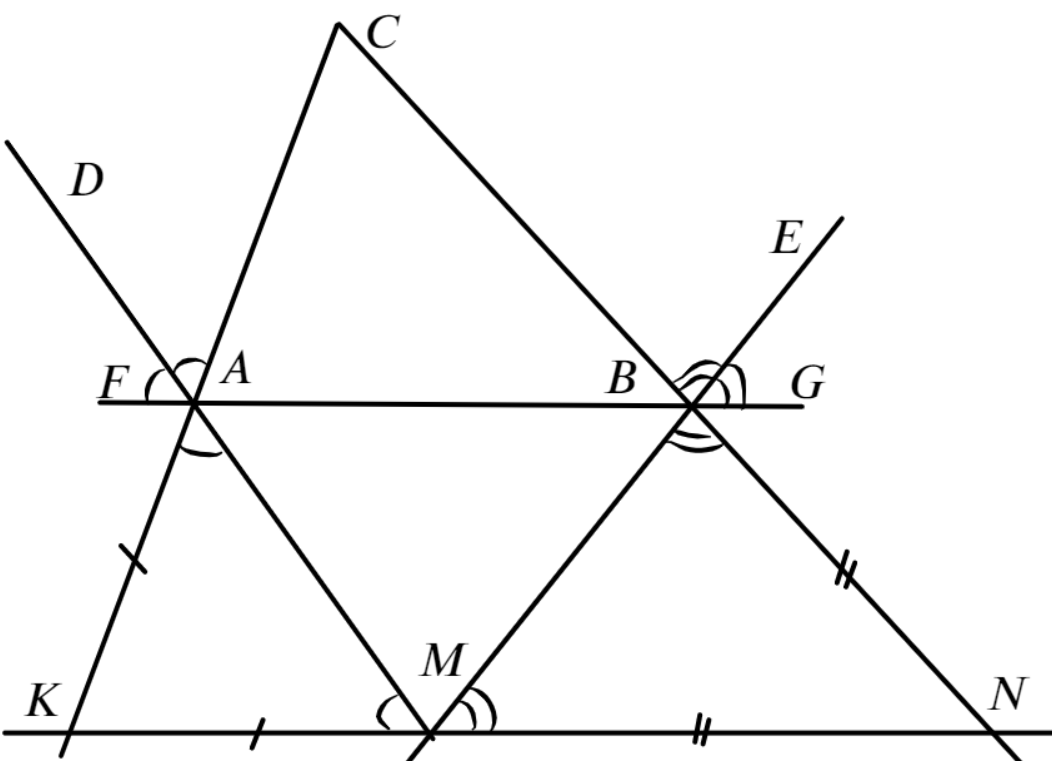
\includegraphics[scale=0.35]{g8-126.png}}
\end{figure}\\
Отметим равные углы, на которые делят угол биссектрисы, вертикальные и накрест лежащие: $\angle MAK=\angle CAD=\angle DAF=\angle AMK$ и $\angle NBM=\angle CBE=\angle EBG=\angle BMN.$ Тогда треугольники $AKM$ и $BNM$ являются равнобедренными и $AK=KM,\ BN=NM.$ Запишем разность $P_{\Delta CKN}-P_{\Delta ABC}=AC+AK+CB+BN+KN-AC-CB-AB=KM+MN+KN-AB=2KN-AB=8-AB=22-18,\ AB=4.$ Но тогда в четырёхугольнике $AKNB$ противоположные стороны $AB$ и $KN$ равны и параллельны, а значит он является параллелограммом и $AK\parallel BN,$ что невозможно (продолжения стороны треугольника не могут быть параллельны). Значит, описанная в задаче ситуация невозможна.
ewpage
oindent
